\documentclass[twoside]{article}

\usepackage{amsmath}
\usepackage{graphicx}


\usepackage[sc]{mathpazo} % Use the Palatino font
\usepackage[utf8]{inputenc}
\usepackage[T1]{fontenc} % Use 8-bit encoding that has 256 glyphs
\linespread{1.05} % Line spacing - Palatino needs more space between lines
\usepackage{microtype} % Slightly tweak font spacing for aesthetics

\usepackage[hmarginratio=1:1,top=32mm,columnsep=20pt]{geometry} % Document margins
\usepackage{multicol} % Used for the two-column layout of the document
\usepackage[hang, small,labelfont=bf,up,textfont=it,up]{caption} % Custom captions under/above floats in tables or figures
\usepackage{booktabs} % Horizontal rules in tables
\usepackage{float} % Required for tables and figures in the multi-column environment - they need to be placed in specific locations with the [H] (e.g. \begin{table}[H])
\usepackage{hyperref} % For hyperlinks in the PDF

\usepackage{lettrine} % The lettrine is the first enlarged letter at the beginning of the text
\usepackage{paralist} % Used for the compactitem environment which makes bullet points with less space between them

\usepackage{abstract} % Allows abstract customization
\renewcommand{\abstractnamefont}{\normalfont\bfseries} % Set the "Abstract" text to bold
\renewcommand{\abstracttextfont}{\normalfont\small\itshape} % Set the abstract itself to small italic text

\usepackage{titlesec} % Allows customization of titles
\renewcommand\thesection{\Roman{section}} % Roman numerals for the sections
\renewcommand\thesubsection{\arabic{subsection}} % Arabic numerals for subsections
\titleformat{\section}[block]{\large\scshape\centering}{\thesection.}{1em}{} % Change the look of the section titles
\titleformat{\subsection}[block]{\large\scshape\centering}{\thesubsection.}{1em}{} % Change the look of the section titles

\usepackage{fancyhdr} % Headers and footers
\pagestyle{fancy} % All pages have headers and footers
\fancyhead{} % Blank out the default header
\fancyfoot{} % Blank out the default footer
\fancyfoot[RO,LE]{\thepage} % Custom footer text

%----------------------------------------------------------------------------------------
%	TITLE SECTION
%----------------------------------------------------------------------------------------

\title{\vspace{-15mm}\fontsize{24pt}{10pt}\selectfont\textbf{Predictive Typing System \\ \fontsize{18pt}{10pt}\selectfont Text Analysis and Retrieval}} % Predictive typing

\author{
\large
\textsc{Mihael Šafarić 0036460167}\\\textsc{Matija Šantl 0036458898}\\
\normalsize Faculty of Electrical Engineering and Computing \\
\vspace{-5mm}
}
\date{}

%----------------------------------------------------------------------------------------

\begin{document}

\maketitle % Insert title

\thispagestyle{fancy} % All pages have headers and footers

%----------------------------------------------------------------------------------------
%	ABSTRACT
%----------------------------------------------------------------------------------------

\begin{abstract}
In this paper we survey two algorithms for smoothing models for language n-gram modeling, Witten-Bell and Kneser-Ney. We implemented simple text editor which uses this methods and then we investigate how factors such as training data size, training corpus, and n-gram order affect to the finally results of this methods which is measured through TODO. We find that these factors can significantly affect the performance of models, especially training data size. TODO Results are showing ...
\end{abstract}

%----------------------------------------------------------------------------------------
%	ARTICLE CONTENTS
%----------------------------------------------------------------------------------------

\begin{multicols}{2}

\section{Introduction}
A language model is a probability distribution p(s) over string s that describes how often the string s occurs as a sentence in some domain of interest. 
Language models provide text entry system with the power to predict unseen text likely to be generated by a user and they are used in many tasks including speech recognition, optical character recognition, handwriting recognition, machine translation, and spelling correction.  That enables people to create text in collaboration with machines which improves efficiency and makes usage of electronic devices more accessible to disabled people. The most commonly used language models are trigram models and they determine the probability of a word given the previous two words, $ p(\omega_i|\omega_{i-2}\omega_{i-1}) $. The simplest way to approximate this probability is to compute 
\begin{equation}
p(\omega_i|\omega_{i-2}\omega_{i-1}) = \frac{c(\omega_{i-2}\omega_{i-1}\omega_i)}{c(\omega_{i-2}\omega_{i-1})}
\end{equation}
where the $ c(\omega_{i-2}\omega_{i-1}\omega_i) $ is the number of times the word sequence $ \omega_{i-2}\omega_{i-1}\omega_i $ occurs in some corpus of training data and $ c(\omega_{i-2}\omega_{i-1}) $ is the number of times word sequence $ \omega_{i-2}\omega_{i-1} $ occurs. This probability is called the maximum likelihood estimate. Maximum likelihood estimate can lead to poor performance in many applications of language models, for example, if the correct transcription of an utterance contains a trigram that has never occur in the training data, we will have $ p_{ML}(\omega_i|\omega_{i-2}\omega_{i-1})=0 $ which will cause the wrong prediction. To address this problem a technique called smoothing was used. The term smoothing describes techniques for adjusting maximum likelihood estimate of probabilities to produce more accurate probabilities. 

In this work, we implemented simple text editor with predictive typing which uses Witten-Bell or Kneser-Ney smoothing technique to predict next word with possibility of choosing which n-gram will be used in this process.  

\section{Methods}

In this section, we survey two smoothing algorithms for n-gram models, Witten-Bell smoothing and Kneser-Ney smoothing. 

The first smoothing algorithm we\rq{}re going to describe is the Witten-Bell smoothing algorithm. Witten-Bell smoothing algorithm is a very simple technique that performs rather poorly \cite{1_chen1999empirical}. Next, we describe the Kneser-Ney smoothing algorithm. Kneser-Ney smoothing works very well and it outperforms Witten-Bell smoothing algorithm.

\subsection{Witten-Bell smoothing}
Witten-Bell smoothing was developed for the task of text compression. The nth-order smoothed model is defined recursively as a linear interpolation between the nrh-order maximum likelihood and the (n-1)th-order smoothed model. The probability of the next word is calculated as

\begin{equation}
p_{WB}(\omega_i|\omega_{i-n+1}^{i-1})=\frac{c(\omega_{i-n+1}^{i}) + N_{1+}(\omega_{i-1}^{i-n+1}\cdot)p{WB}(\omega_i|\omega_{i-n+2}^{i-1})}{\sum_{wi}c(\omega_{i-n+1}^{i}) + N_{1+}(\omega_{i-1}^{i-n+1}\cdot)}
\end{equation}

\subsection{Kneser-Ney smoothing}
Kneser-Ney smoothing algorithm was introduced in 1995. as an extension of absolute discounting where the lower-order distributions that one combines with a higher-order distribution is built in a novel manner \cite{1_chen1999empirical}. 

Next we\rq{}ll present the mathematical background of the Kneser-Ney smoothing algorithm.

Considering bigram models, we would like to select a smoothed distribution $p_{KN}$ that satisfies the following constraint on unigram marginals for all $w_i$:

\begin{equation}
\sum_{w_{i - 1}} p_{KN}(w_{i-1}w_{i} ) = \frac{c(w_{i})}{\sum_{w{i}} c(w_{i})}
\end{equation}
where the function $c(w_{i})$ denotes the count of the word $w_{i}$ in the given corpus. The left hand-side of this equation is the unigram marginal for $w_{i}$ of the smoothed bigram distribution $p_{KN}$, and the right-hand side is the unigram frequency of $w_{i}$ found in the given corpus.

As in absolute discounting where $0 \le D \le 1$, we assume that the model has the following form:

\begin{multline}
p_{KN}(w_{i} | w_{i-n+1}^{i-1}) = \frac{max(c(w_{i-n+1}^{i}) - D, 0)}{\sum_{w_{i}} c(w_{i-n+1}^{i})}  \\ + \frac{D}{\sum_{w_{i}} c(w_{i-n+1}^{i})} N_{1+}(w_{i-n+1}^{i-1} \cdot) p_{KN}(w_{i} | w_{i-n+2}^{i-1}) 
\end{multline}
where 
\begin{equation}
N_{1+}(\cdot w_{i}) = |{w_{i} : c(w_{i-1}w_{i}) > 0}|
\end{equation}

is the number of different words $w_{i-1}$ that precede $w_{i}$ in the given corpus.

We used this formulation, because as stated in \cite{1_chen1999empirical}, it leads to a cleaner derivation of essentially the same formula; no approximations are required, unlike in the original derivation.

By applying the law of total probability, we can write equations given above as following:
\begin{equation}
p_{KN}(w_{i-1}w_{i} ) = \sum_{w_{i-1}} p_{KN}(w_{i} | w_{i-1} )p(w_{i-1})
\end{equation}
which leads to:

\begin{equation}
\frac{c(w_{i})}{\sum_{w{i}} c(w_{i})} = \sum_{w_{i-1}} p_{KN}(w_{i} | w_{i-1} )p(w_{i-1})
\end{equation}

Taking into account that $p(w_{i-1}) =\frac{c(w_{i-1})}{\sum_{w{i-1}} c(w_{i-1})} $, we have
\begin{equation}
c(w_{i}) = \sum_{w_{i-1}} c(w_{i-1}) p_{KN}(w_{i} | w_{i-1})
\end{equation}

which, after substituting and simplifying leads to the following form:

\begin{equation}
c(w_{i}) = c(w_{i}) - N_{1+}(\cdot w_{i}) + D p_{KN}(w_{i}) \sum_{w_{i}} N_{1+}(\cdot w_{i})
\end{equation}

Generalizing to higher-order models, we have the final form for the word probability:

\begin{equation}
p_{KN}(w_{i} | w_{i-n+2}^{i-1}) = \frac{N_{1+}(\cdot w_{i-n+2}^{i})}{\sum_{w_{i}}N_{1+}(\cdot w_{i-n+2}^{i})} 
\end{equation}

\section{Results}
Implemented language models with Witten-Bell and Kneser-Ney smoothing algorithms were evaluated using measures of perplexity and cross-entropy on separete fractions of the test corpus. Finally, a \nameref{image:editor} with the predicting capabilities was developed.

\subsection{Evaluation}

\subsection{Text editor}

\section{Discussion}

\section{Conclusion}
TODO U 2... u Introduction ima zakaj je predictin typing dobar, a zakaj ne

%----------------------------------------------------------------------------------------
%	REFERENCE LIST
%----------------------------------------------------------------------------------------

\bibliography{bibliography}{}
\nocite{*}
\bibliographystyle{abbrv}

%----------------------------------------------------------------------------------------

\end{multicols}

\appendix
\section{Text Editor}

\begin{figure}[hT!]
        \label{image:editor}
        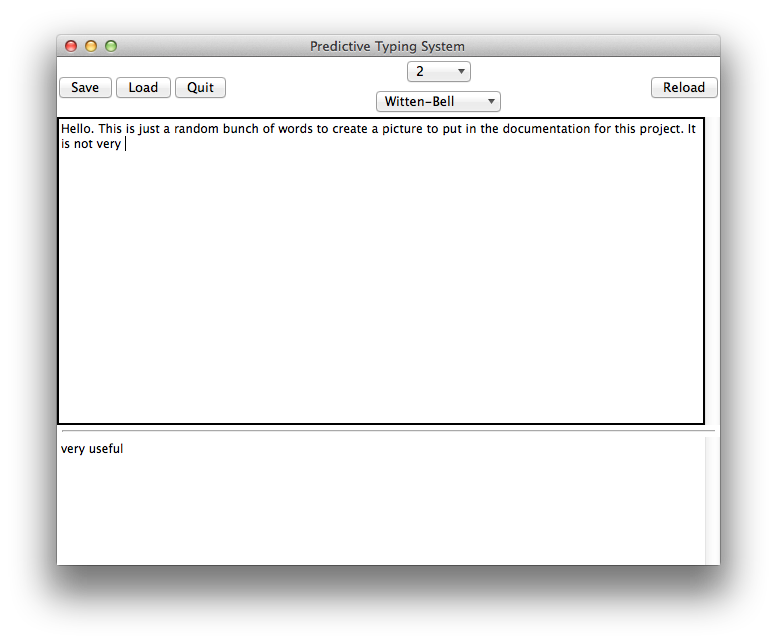
\includegraphics[width=\textwidth]{editor.png}
        \caption{Text editor}
\end{figure}

\end{document}
